\section{Motivation}\label{sec:motivation}
In this section we describe the processes of Authentication and Authorization in the system.
It is worth to remember the meaning of Authentication and Authorization definitions.
Authentication -- is the process of ascertaining that somebody really is who they claim to be [\cite{burrows1989logic}].
Authorization refers to rules that determine who is allowed to do what [\cite{fagin1978authorization}].
For example, Adam may be authorized to create and delete databases, while Eve is only authorized to read.
The two concepts are completely orthogonal and independent, but both are central to security design, and the
failure to get either one correct opens up the avenue to compromise.
In terms of web apps, very crudely speaking, authentication is when you check login credentials to see if you recognize
a user as logged in, and authorization is when you look up in your access control whether you allow the user to view,
edit, delete or create content.
As to the projects concerns, we should handle multiple client applications, e.g desktop,
web, mobile etc.
Therefore, cookie authorization doesn't fit for the project, however the JWT one surely passes.


\section{JWT Tokens}\label{sec:jwt-tokens}
So, what is JSON Web Token (JWT)?
JSON Web Token (JWT) is an open standard (RFC 7519) that defines a compact and self-contained way for securely
transmitting information between parties as a JSON object [\cite{jones2015json}].
This information can be verified and trusted because it is digitally signed.
JWTs can be signed using a secret (with the HMAC algorithm [\cite{wang2004hmac}]) or a public/private key pair using RSA or ECDSA\@.
Although JWTs can be encrypted to also provide secrecy between parties, we will focus on signed tokens.
Signed tokens can verify the integrity of the claims contained within it, while encrypted tokens hide those claims from
other parties.
When tokens are signed using public/private key pairs, the signature also certifies that only the party holding the
private key is the one that signed it.
In its compact form, JSON Web Tokens consist of three parts separated by dots, which are:
\begin{itemize}
    \item Header -- typically consists of two parts: the type of the token, which is JWT, and the signing algorithm
    being used, such as HMAC SHA256 or RSA\@.
    \item Payload -- The second part of the token is the payload, which contains the claims.
    Claims are statements about an entity (typically, the user) and additional data.
    There are three types of claims: registered, public, and private claims.
    \item Signature -- To create the signature part you have to take the encoded header, the encoded payload, a secret,
    the algorithm specified in the header, and sign that.
\end{itemize}
Therefore, a JWT typically looks like \texttt{xxxxx.yyyyy.zzzzz}.
Then, this JSON is Base64Url encoded to form the first part of the JWT\@.


\section{JWT Authentication}\label{sec:jwt-authentication}
An authentication, when the user successfully logs in using their credentials, a JSON Web Token will be returned.
Since tokens are credentials, great care must be taken to prevent security issues.
In general, you should not keep tokens longer than required.
You also should not store sensitive session data in browser storage due to lack of security.
Whenever the user wants to access a protected route or resource, the user agent should send the JWT,
typically in the Authorization header using the Bearer schema.
The content of the header should look like \texttt{Authorization: Bearer <token>}.
This can be, in certain cases, a stateless authorization mechanism.
The server's protected routes will check for a valid JWT in the Authorization header, and if it's present, the user
will be allowed to access protected resources.
If the JWT contains the necessary data, the need to query the database for certain operations may be reduced, though
this may not always be the case.
If the token is sent in the Authorization header, Cross-Origin Resource Sharing (CORS) won't be an issue as it doesn't
use cookies.
The following diagram shows how a JWT is obtained and used to access APIs or resources:
\begin{figure}[H]
    \centering
    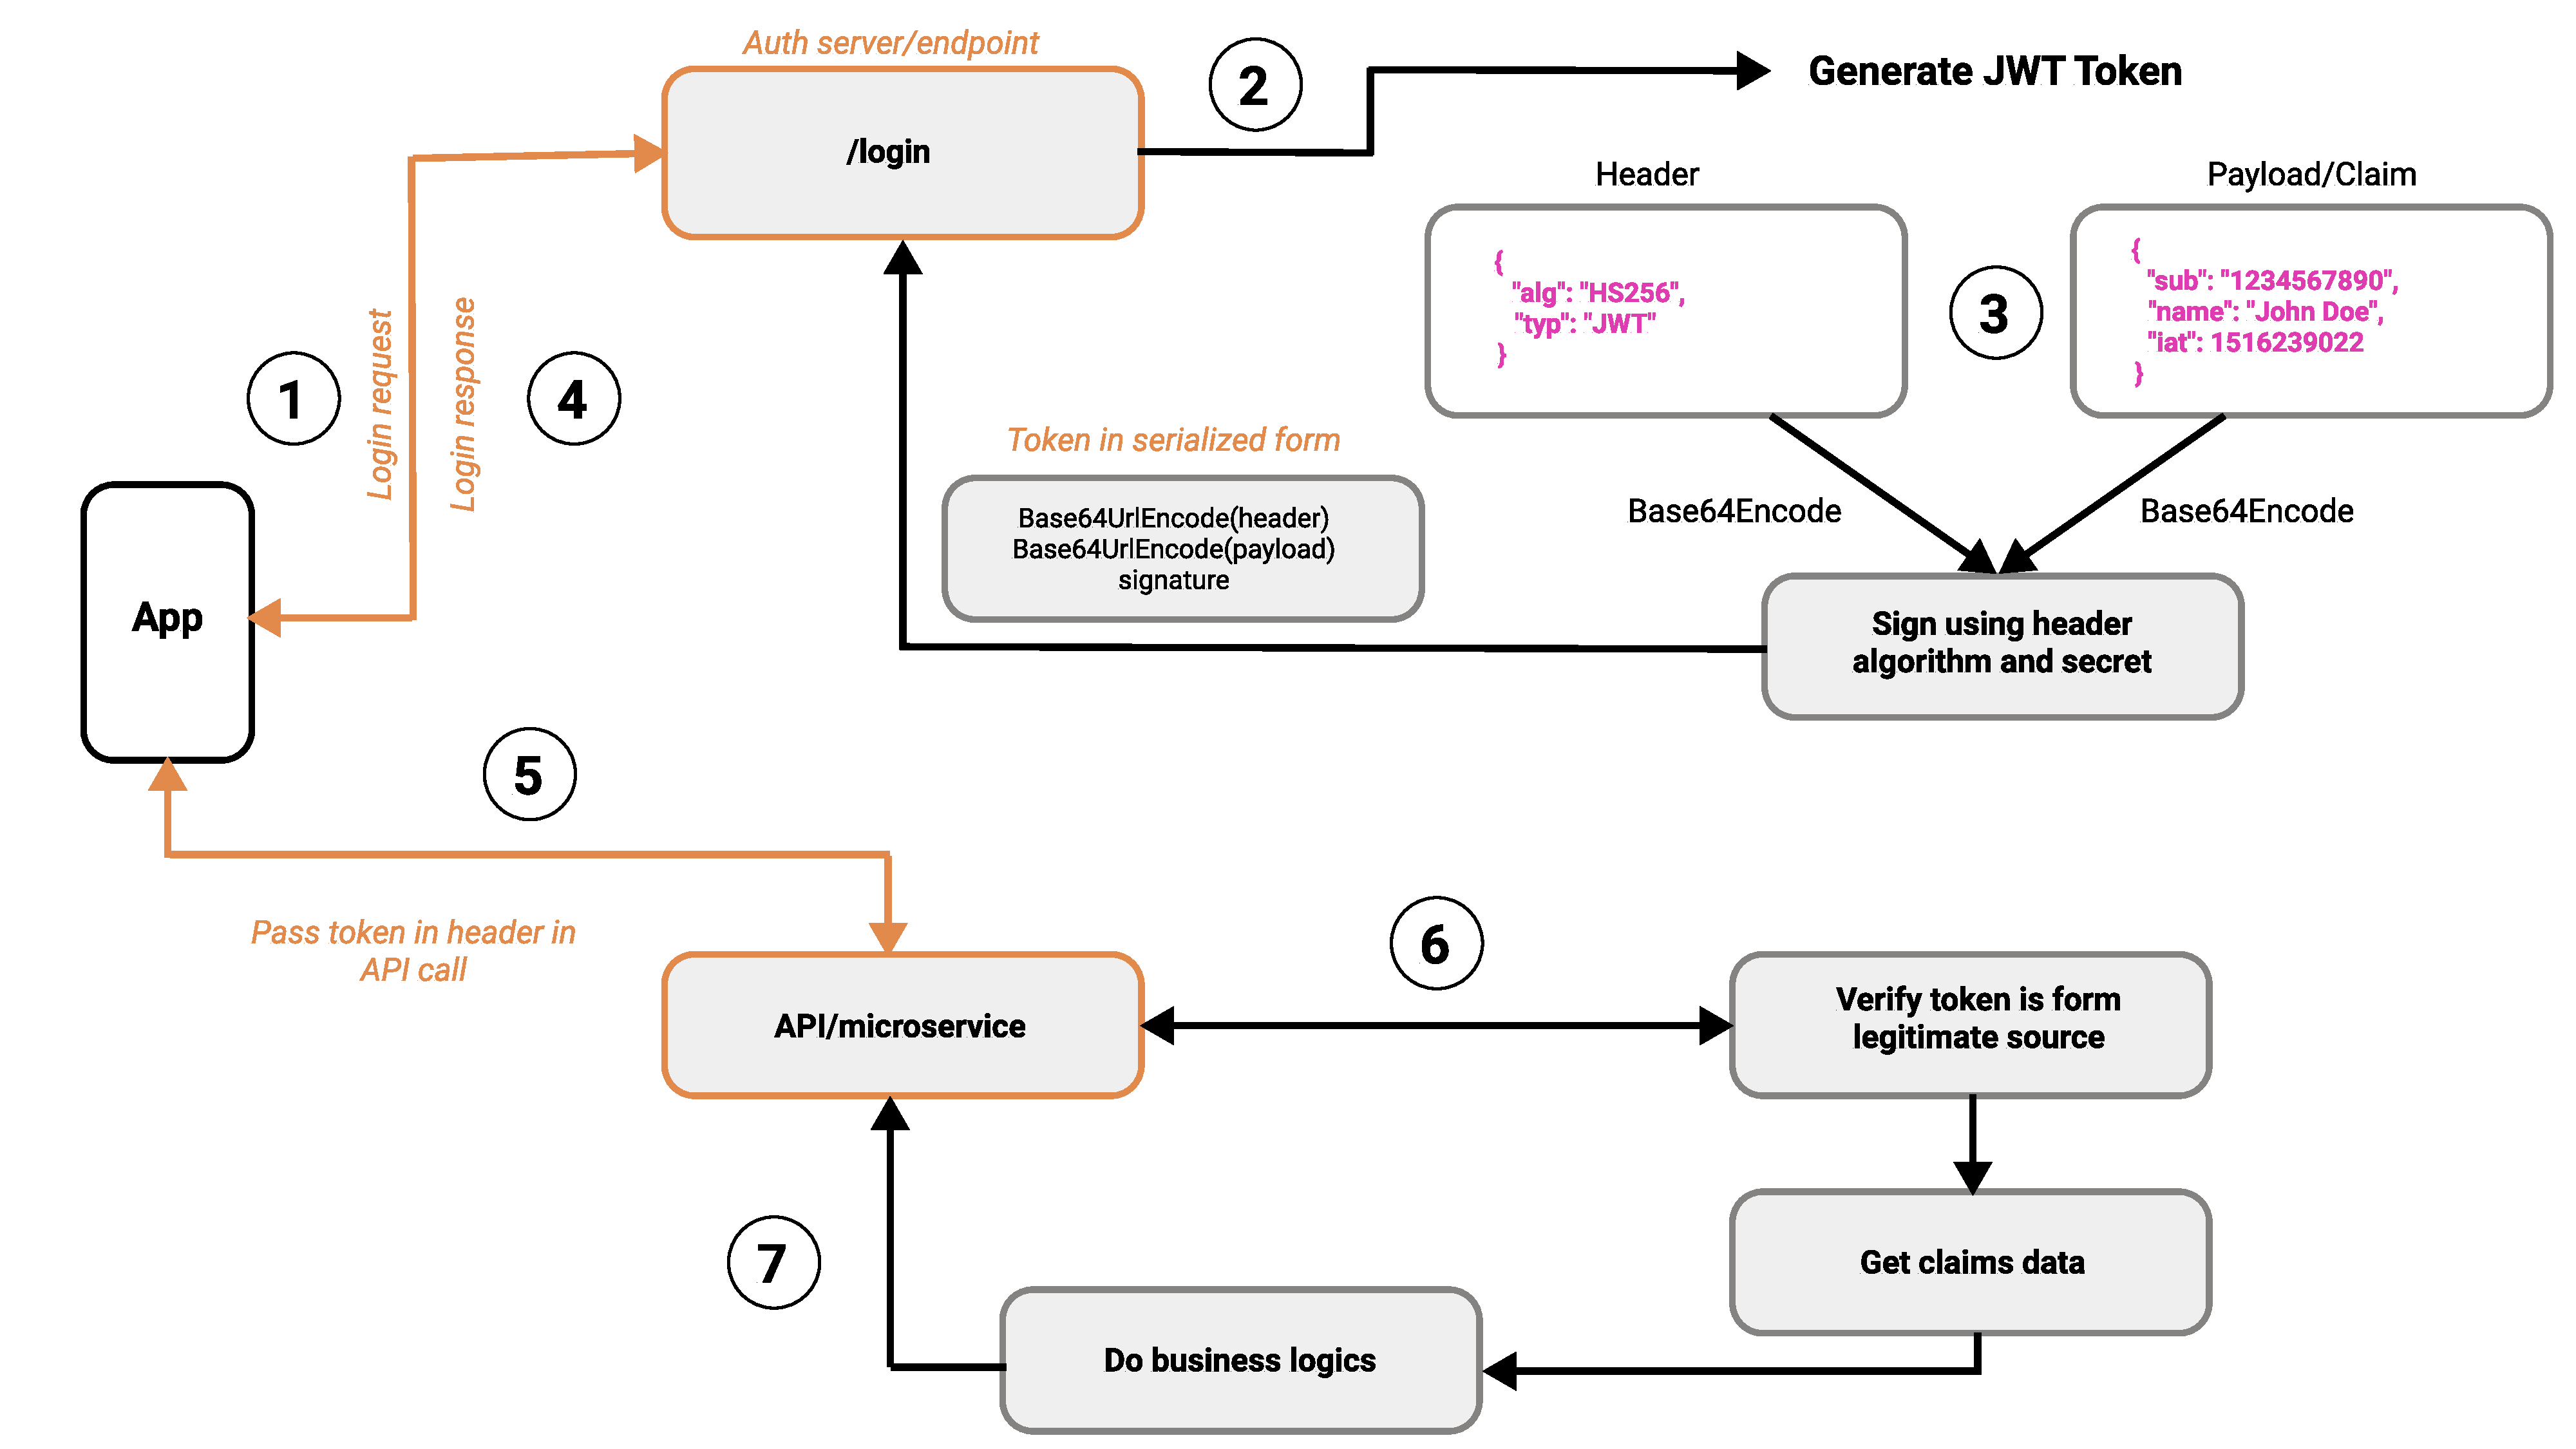
\includegraphics[width=1\textwidth]{Pictures/jwt_auth_scheme.pdf}
    \caption{JWT Authentication principle diagram.}\label{fig:figure3}
\end{figure}
JWT is quite simple and straightforward way to authorize particular person to the system's part.
However, what is about security, does it provide enough level of security?
Not really is.
When the JWT token is stolen, there is no way to revoke it.
Only the thing is to wait while token expires by himself, after its predefined lifetime.
A few basic rules about JWT usage [\cite{RDegges}]
\begin{itemize}
    \item JWT should have a short lifetime (few seconds).
    \item JWT should be used in a single time, e.g JWT per request.
\end{itemize}